\section{Why the model gives minutes to liner loss}\label{sec:caloric}
When the liner disappears, every kilogram of initial phenolic has passed through
pyrolysis. In the specified chemistry, a fraction $y=0.48$ of that mass becomes
char and eventually leaves through the hot surface. For original hot radius $r_i$,
thickness $d$ and exposed area $A_0$, the original virgin mass per area follows
from the volume of the annulus. The model's total chemical energy cost is then
\[
  \frac{m_0}{A_0}=\rho_v d\left(1+\frac{d}{2r_i}\right),\qquad
  \frac{E_{\rm chem}}{A_0}=\frac{m_0}{A_0}(L_p+yL_c).
\]
The assumed costs are $L_p=0.418$ MJ per kg of virgin phenolic and $L_c=35$ MJ
per kg of expelled char. They give 108.7 and 143.3 MJ/m$^2$ for the sustainer
and booster, respectively. The calculation accounts separately for the sensible
heat leaving with reaction products, the heat retained by the casing and the
heat lost to ambient. For CF it also includes gas enthalpy and net resin reaction
energy.
\begin{figure}[H]\centering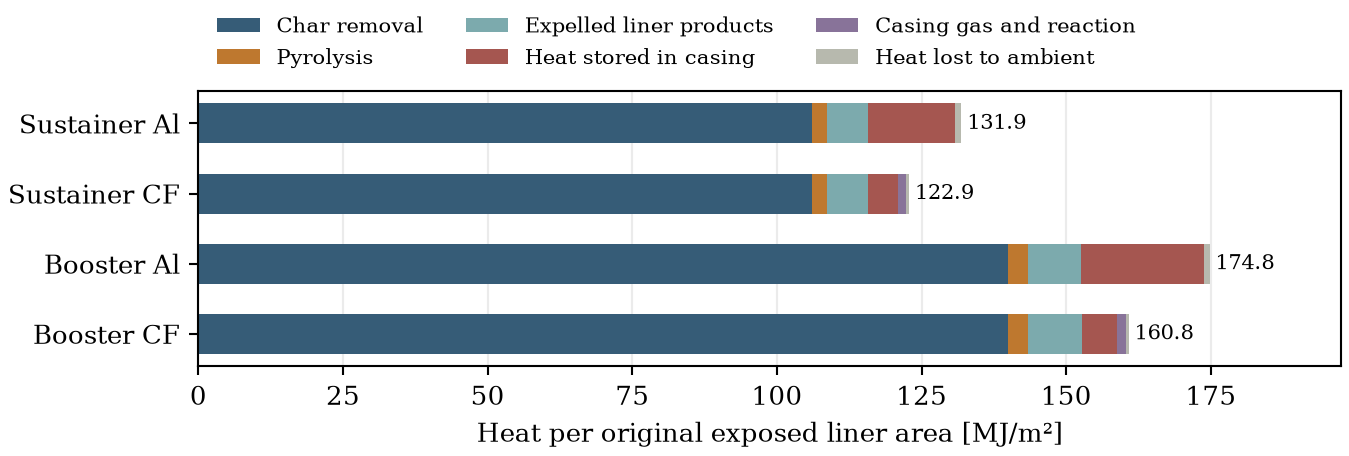
\includegraphics[width=0.97\textwidth]{../analysis/liner_energy_inventory.png}
\caption{Energy delivered by the film through complete liner loss at nominal heating.
The Al storage term includes fusion. The four bar totals use the same original-area
basis as the chemical energy calculation. Both backing surrogates retain their shape.}
\end{figure}
For the sustainer Al example, the computed film delivers 131.9 MJ/m$^2$ at
a time-average rate of 1.194 MW/m$^2$ on the original area. Their ratio is
110.5 s. The mean on the moving area in the preceding section is smaller
because that area grows. This division explains the solved duration. Both the
dose and the incident power come from the transient solution.

Across all twelve cases, 79.7--87.3\% of incident energy pays the assumed
char-removal cost. The two numerical methods agree on total dose to within
0.044\%. A measured mass-loss and recession history under a known heat load
would test the effective cost and the prescribed char yield. Their product sets
the largest term in this estimate.

\paragraph{Gas and solid temperature.} The prescribed gas temperature is
2504 K (2231 $^\circ$C). Across the four motors the highest saved live hot-face
temperatures are 975--988, 1082--1083 and 1229--1232 $^\circ$C at the weaker, nominal
and stronger film coefficients respectively. These are maxima of the saved surface
samples. The burning gas, the exposed char and the casing interface have separate
temperatures.
\clearpage
